\documentclass[a4paper,12pt,titlepage,final]{article}

\usepackage{amsmath}
\usepackage{amsfonts}
\usepackage{amssymb}\usepackage{amssymb}
\usepackage{csvsimple}
\usepackage{tikz}
\usepackage{pgfplots} \pgfplotsset{compat=1.18}
\usepackage{cmap}
\usepackage{color}
\usepackage[utf8]{inputenc}
\usepackage[T2A]{fontenc}
\usepackage[english,russian]{babel}
\newcommand{\gt}{\textgreater} % знак больше
\newcommand{\lt}{\textless}       % знак меньше]
\usepackage[margin=2cm]{geometry}		 % для настройки размера полей
\usepackage{indentfirst}         % для отступа в первом абзаце секции
\usepackage{amsmath}
\usepackage{fancyvrb}
\usepackage{listings}
\usepackage{bm}
\usepackage{float}
\usepackage{hyperref}

\usepackage[nottoc,numbib]{tocbibind}
\usepackage{blindtext}
\usepackage{array}
\sloppy

% выбираем размер листа А4
\geometry{a4paper,left=30mm,top=20mm,bottom=20mm,right=10mm}

%\setcounter{secnumdepth}{0}      % отключаем нумерацию секций

\newenvironment{compactlist}{     % перечисление без больших интервалов
\begin{list}{{$\bullet$}}{
\setlength\partopsep{0pt}
\setlength\parskip{0pt}
\setlength\parsep{0pt}
\setlength\topsep{0pt}
\setlength\itemsep{0pt}
}
}{
\end{list}
}

\begin{document}

\begin{titlepage}
  \begin{center}

    
\includegraphics[scale=0.2]{gzlogo}\\
    \small
    \centerline{Московский государственный университет имени М.В. Ломоносова}
    \centerline{Факультет вычислительной математики и кибернетики}
    \centerline{Кафедра автоматизации систем вычислительных комплексов}
    \centerline{}

    
    \Large
    \vfill
    {Отчет по заданию практикума}\\
    {\LARGE \bf
      Генетический алгоритм
    }\\
    \null \null
    
  \end{center}
  
  \begin{flushright}
    {\bf Выполнил:}\\
    Бритенков Егор Сергеевич, 421 группа\\
    \vfill
  \end{flushright}

\centerline{Москва, 2023}
\end{titlepage}

\tableofcontents
\newpage

\begin{section}{Введение}

    C помощью генетического алгоритма решить задачу:

    Найти начальную конфигурацию "<Game of Life"> поля размером 50х50, минимизирую требуемый критерий.

    \textbf{Критерий:} количество заполненных клеток после 100 шагов клеточного автомата (т.е. в 101-й конфигурации, в нумерации с 1).
    
    \textbf{Ограничение:} конфигурация, возникающая после 100 шагов клеточного автомата, не является стационарной. То есть её потомок (результат следующего шага клеточного автомата) не совпадает с ней.

    \textbf{Детализация алгоритма:}
    \begin{compactlist}
        \item Функция выживаемости: значение оптимизируемого критерия + возможный штраф.
        \item Решение~--- битовый вектор
        \item Размер популяции 100
        \item Для селекции использовался бинарный турнирный алгоритм
        \item Использовалось одноточечное скрещивание
        \item Вероятность скрещивания 0.8
        \item Начальная популяция: полностью случайно генерируется, вероятность того, что в клетке 1 равна 0.5.
        \item Критерий останова: 50 итераций ГА (т.е. 50 смен популяций) подряд без улучшения значения оптимизируемого критерия на лучшем из найденных решений.
        \item Решения, не удовлетворяющие ограничению, штрафуются.
        \item Операция мутации стандартная, вероятность мутации перебирается в ходе исследования.
    \end{compactlist}

\end{section}

\begin{section}{Исследование реализации}
    \textbf{Задание:} необходимо исследовать зависимость характеристик работы алгоритма от интенсивности мутации, т.е. от значения $P_{mut}$. 
    Начальное значение $P_{mut}$: $P_{mut\_init} = \frac{1}{50 * 50} = 0.0004$, т.е. в среднем в каждом решении мутирует 1 бит.

    Изменять $P_{mut}$ в ходе исследования следует по формуле: $P_{mut}(i) = P_{mut\_init} * 1.5^i, i = 0,\ldots,9$; i – номер серии экспериментов, т.е. нужно провести 10 серий экспериментов, каждая со своим фиксированным значением $P_{mut}$. Например, в серии 3 $P_{mut}=P_{mut}(3)=0.0004*(1.5^3)=0.00135$.
    
    Для каждого значения i необходимо провести серию из 10 запусков ГА с соответствующим значением $P_{mut} = P_{mut}(i)$ и определить:
    \begin{itemize}
        \item Стабильность алгоритма (разброс значений критерия на решении-результате, т.е. разность между значениями критерия на худшем и на лучшем прогоне)
        \item Качество работы алгоритма (значение критерия на лучшем прогоне)
        \item Вычислительные затраты на выполнение алгоритма (количество процессорного времени, затраченного на прогон; брать максимум по 10 прогонам)
    \end{itemize}

\newpage
    
    \begin{subsection}{Стабильность}
    
    \begin{figure}[H]
    	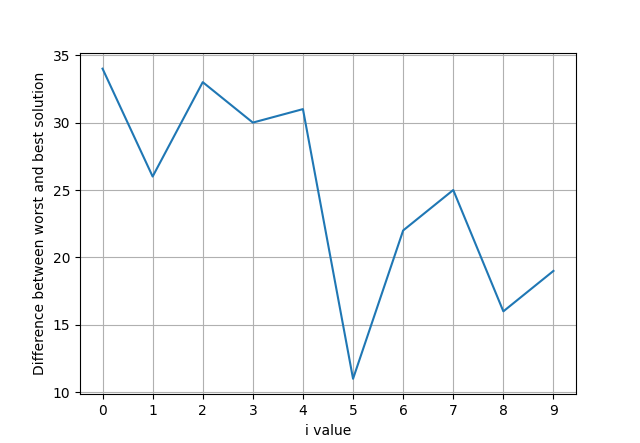
\includegraphics[width=17cm]{1.png}
    	\label{pic:2}
    \end{figure}

    Стабильность в целом увеличивается (т.е. разница между лучшим и худшим решениями уменьшается) с увеличением вероятности мутации. Оптимальным является значение на серии 5. На графике значение разности между значениями лучшего найденного решения и худшего.
    \end{subsection}

    \newpage

    \begin{subsection}{Качество}
    
    \begin{figure}[H]
    	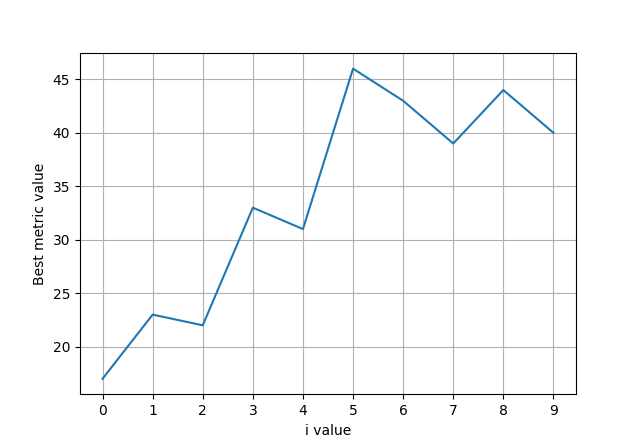
\includegraphics[width=17cm]{2.png}
    	\centering
    	\label{pic:1}
    \end{figure}

    Качество с увеличением вероятности мутации падает (т.е. значение наилучшего полученного критерия увеличивается). Наилучшее решение также получено на серии 5.
    \end{subsection}

    \newpage

    \begin{subsection}{Вычислительные затраты}

    \begin{figure}[H]
    	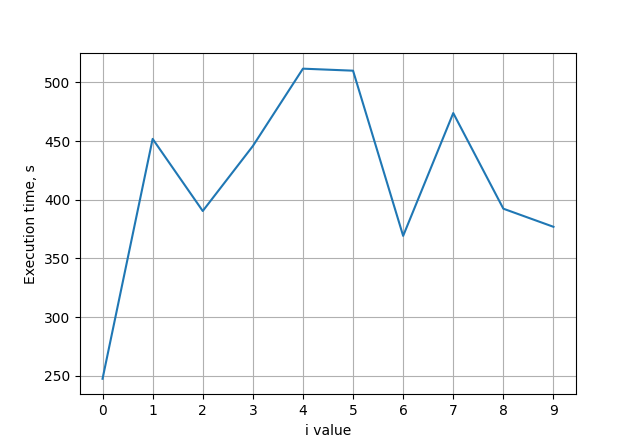
\includegraphics[width=17cm]{3.png}
    	\label{pic:3}
    \end{figure}

    Судя по полученному графику, время поиска решения не вполне зависит от вероятности мутации.
    \end{subsection}
\end{section}

\begin{section}{Выводы}

    Судя по полученным графикам, с увеличением вероятности мутации алгоритм приходит к более случайным решениям, из-за этого получая худшие и более близкие по значению критерия решения. При небольших же значениях вероятности мутации алгоритм сходится более "<планомерно"> при удачных входных данных и менее при неудачных.
    
\end{section}

\end{document}
